\documentclass[oneside,a4paper,11pt]{kth-mag}
\usepackage[T1]{fontenc}
\usepackage{textcomp}
\usepackage{lmodern}
\usepackage[utf8]{inputenc}
\usepackage[swedish,english]{babel}
\usepackage{modifications}
\usepackage{listings}
\usepackage{hyperref}
\usepackage{graphicx}
\usepackage[figuresleft]{rotating}
\usepackage{geometry}
\title{Modular responsive web design}

\subtitle{Allowing responsive web modules to respond to custom criterias instead of only viewport size by implementing \emph{element queries}}
\author{Lucas Wiener \\ \lowercase{lwiener@kth.se}}
\date{February 2015}
\blurb{Master's Thesis task specification\\\hfill\\ Supervisors at \textsc{evry ab}: Tomas Ekholm \& Stefan Senner\"{o}\\Supervisor at \textsc{csc}: Philipp Haller\\Examiner: Mads Dam}
\trita{February 2015}
\begin{document}
\frontmatter
\pagestyle{empty}
\removepagenumbers
\maketitle
\mainmatter
\section*{Problem definition}
By using \textsc{css} \emph{media queries} developers can specify different rules for different viewport sizes. This is fundamental to create responsive web applications. If developers want to build modular applications by composing the application by smaller components (elements, scripts, styles, etc.) the media queries are no longer applicable. Modular components should be able to react and change style depending on the given size that the component has been given by the application, not the viewport size. The problem can be formulated as: \emph{Elements can not specify conditional style rules depending on their own size, or the size of any other element}.

\textsc{w}\oldstylenums{3}\textsc{c}\footnote{World Wide Web Consortium (abbreviated \textsc{w}\oldstylenums{3}\textsc{c}) is the main international standards organization for the World Wide Web.} has unofficially stated that such feature would be infeasible to implement. Some problems with implementing element queries in \textsc{css} are:
\begin{itemize}
    \item \textbf{Circularity:} The styling of elements depend on many factors (theoretically on all other elements in the layout tree). If elements can apply styles by criterias of other elements, it will be possible to create infinite loops of styling. The simplest example of this would be an element to set its width to 200 pixels if it is under 100 pixels wide. If the element is under 100 pixels wide, the new style will be applied to the element which would make the width of the element 200 pixels. If this element would have another rule that set its width to 50 pixels if it is wider than 150 pixels, there is an infinite loop of styling. Problems like this can probably be catched during \textsc{css} parsing, but there are so many combinations of style properties that could result in similar loops that it will add a lot of complexity to the language, both for implementers and users.
    \item \textbf{Performance:} Rendering engines typically perform selector matching and layout computations in parallel to achieve good performance. If element queries would be implemented, the rendering engines would need to first compute the layout of all elements in order to decide which selectors would conform to the element query conditions and then do a new layout computation, and so on until a stable state has been reached. Far worse, since selectors now depend on layout style, this cannot be done in parallel which impacts performance heavily.
\end{itemize}
Because of the problems, it is stated that such feature will not be implemented in the near future. So it is now up to the developers to implement this feature as a third-party solution. Efforts have been made by big players to create a robust implementation, with moderate success. Since all implementations have shortcomings, there is still no de facto solution that developers use and the problem remains unsolved.

\section*{Objective}
The main objective of my master's thesis is to develop a third-party implementation of element queries (or equivalent to solve the problem of modular responsive elements). To do this, I will need to research and understand all existing attempts and analyze the advantages and shortcomings of each approach. I will also need to be aware of the premises, such as browser limitations and specifications that need to be conformed. In addition, I will research the problems of implementing element queries natively to get a deeper understanding of how an official \textsc{api} would look like. There are many challenges along the way that will need to be researched and worked around. Examples of such subproblems that would need to be investigated are:
\begin{itemize}
\item How should circularity be handled? Should it be detected at runtime or parsetime, and what should happen on detection?
\item How can one listen to element dimension changes without any native support?
\item How can a custom \textsc{api} be crafted that will enable element queries and still conform to the \textsc{css} specification?
\item If a custom \textsc{api} is developed, how would one make third-party modules (that uses media queries) work without demanding a rewrite of all third-party modules?
\end{itemize}
The scientific question to be answered is if it is possible to solve the problem  without extending the current web standard. The hypothesis is that the problem can be solved in a reliable and performant way by crafting a third-party implementation. A reliable implementation should also enable existing responsive components to react to a specified criteria (parent container size for example) with no modifications to the components. The goal of the thesis should be considered fulfilled if a solution was successfully implemented or described, or if the problems hindering a solution are thoroughly documented.

\section*{Significance}
Web developers are today limited to writing big applications in an entagled mess. In almost all other programming environments it is possible and encouraged to write applications in smaller parts (or modules). By creating modules that can be used in any context with well defined responsibilities and dependencies, developing applications is reduced to the task of simply configuring modules (to some extent) to work together which forms a bigger application. It is today possible to write the web client logic in a modular way in JavaScript. The desire of writing modular code can be shown by the popularity of frameworks that helps dividing up the client code into modules. The ever so popular frameworks Angular, Backbone, Ember, Web Components, requirejs, Browserify, Polymer, React and many more all have in common that they embrace coding modular components. Many of these frameworks also help with dividing the \textsc{html} up into modules, creating small packages of style, markup and code. One of the biggest issues keeping the modules from being truly modular is that they cannot adapt to given sizes. This makes the modules either force the client to style them properly depending on viewport size, or not being responsive. Both options are undesirable for developing larger applications. A third option would be to make the modules context aware and style themselves according to the viewport, which defeats the purpose of modules (making them not reusable).

The last couple of years a lot of articles have been written about the problem and how badly we need element queries. As already stated, third-party implementation efforts have been made by small and big players, with moderate success. \textsc{w}\oldstylenums{3}\textsc{c} keep getting requests and questions about it, but the answer seems to lean towards no. An organization called Responsive Issues Community Group (abbreviated \textsc{ricg}) have started an initial planning regarding element queries. However, things are moving slow and a draft about element queries use cases are still being made.

Solving this problem would be a big advancement to web development, enabling developers to create truly modular components. By studying the problem, identifying approaches and providing a third-party solution the community can take a step closer to solve the problem. If the hypothesis holds, developers will be able to use element queries in the near future, while waiting for \textsc{w}\oldstylenums{3}\textsc{c} to make their verdict. The outcome of this thesis can also be helpful for \textsc{w}\oldstylenums{3}\textsc{c} and others to get an overview of the problem and possibly get ideas how subproblems can be handled.

\section*{Literature study}
Since the problem is relatively new and unique for the web, my main literature will be web articles and \textsc{w}\oldstylenums{3}\textsc{c} mailing lists. There are many experienced individuals writing good articles about the problem and mostly discusses how an \textsc{api} can look like. The \textsc{w}\oldstylenums{3}\textsc{c} mailing lists are a good resource to get insight into how the browser vendors view the problem. To investigate third-party implementation approaches, I will read the implementation attempts that I can find. To understand the issues with implementing the problem better, I will read books, scientific papers and articles covering how rendering engines work. To solve the circular problems of the third-part implementation I will read scientific papers and articles how other languages have solved similar problems. To make sure I fully understand responsive web development I will read books about the subject. To support my claims that modular development is a good thing, I will research scientific papers and books.

\subsection*{Current literature}
\emph{The following is the literature that has been gathered so far.}
\subsubsection*{Books}
\begin{itemize}
\item Tim Kadlec. Implementing Responsive Design: Building sites for an anywhere, everywhere web. New Riders, 2012.
\item Frain, Ben. Responsive Web Design with HTML5 and CSS3. Packt Publishing, 2012.
\item Scott Jehl. Responsible Responsive Design. A Book Apart, 2014.
\end{itemize}
\subsubsection*{Scientific papers and reports}
\begin{itemize}
\item Jerjas, Allan. Building Blocks of Responsive Web Design. KTH, 2013. URN: \url{urn:nbn:se:kth:diva-142345}
\item Tobias Sundqvist, Christoffer Wåhlander. Applikationsutveckling i Responsive Web Design. LIU, 2013. ISRN: \url{LIU-IDA/LITH-EX-G--13/011--SE}
\item Christopher Grant Jones, Rose Liu, Leo Meyerovich, Krste Asanovic, Rastislav Bodík. Parallelizing the Web Browser. In Proceedings of the First USENIX Workshop on Hot Topics in Parallelism. Department of Computer Science, University of California, Berkeley, 2009.
\item Calin Cascaval, Seth Fowler, Pablo Montesinos Ortego, Wayne Piekarski, Mehrdad Reshadi, Behnam Robatmili, Michael Weber, Vrajesh Bhavsar. ZOOMM: A Parallel Web Browser Engine for Multicore Mobile Devices. In Principles and Practice of Parallel Programming. Qualcomm Research Silicon Valley, 2013.
\item Alan Grosskurth, Michael W. Godfrey. Architecture and evolution of the modern web browser. In Proceedings of the 21st IEEE international conference on software maintenance (ICSM'05). David R. Cheriton School of Computer Science, University of Waterloo, Waterloo, ON N2L 3G1, Canada, 2006.
\item Helen J. Wang, Chris Grier, Alexander Moshchuk, Samuel T. King, Piali Choudhury, Herman Venter. The Multi-Principal OS Construction of the Gazelle Web Browser. In USENIX security symposium (Vol. 28). Microsoft Research, University of Illinois at Urbana-Champaign, University of Washington, 2009.
\item Lingjun Fan, Weisong Shi, Shibin Tang, Chenggang Yan2 Dongrui Fan. Optimizing web browser on many-core architectures. In Parallel and Distributed Computing, Applications and Technologies (PDCAT), 2011 12th International Conference. Chinese Academy of Sciences, Wayne State University, 2011.
\item Carmen Badea, Mohammad R. Haghighat, Alexandru Nicolau, Alexander V. Veidenbaum. Towards Parallelizing the Layout Engine of Firefox. In Proceedings of the 2nd USENIX conference on Hot topics in parallelism. UC Irvine, Intel Corporation, 2010.
\end{itemize}
\subsubsection*{Articels}
\begin{itemize}
\item Tali Garsiel, Paul Irish. How Browsers Work: Behind the scenes of modern web browsers. html5rocks, 2011. \url{http://www.html5rocks.com/en/tutorials/internals/howbrowserswork/}
\item Dave Hyatt. Layout and Rendering. The WebKit Open Source Project, 2007. \url{http://www.webkit.org/projects/layout/index.html}
\end{itemize}

\subsubsection{Other}
\begin{itemize}
\item Francois Remy. The :min-width/:max-width pseudo-classes. \textsc{w}\oldstylenums{3}\textsc{c} mailing list, 2013. \url{https://lists.w3.org/Archives/Public/www-style/2013Mar/0368.html}
\item Kevin Mack. Element Query and Selector Media Query Types. \textsc{w}\oldstylenums{3}\textsc{c} mailing list, 2014. \url{https://lists.w3.org/Archives/Public/public-respimg/2014Oct/0005.html}
\item Responsive Issues Community Group element queries use discussion repository. \url{https://github.com/ResponsiveImagesCG/eq-usecases}. Creating the use cases draft: \url{https://responsiveimagescg.github.io/eq-usecases/}
\end{itemize}

In addition to the listed literature, numerous web articles has been found regarding element queries. There are around 10 unique open source implementation attempts of element queries to examine. No good in-depth literature regarding rendering engines and why element queries are hard to implement natively has yet to be found.

The literature study will be examined by a verbal presentation to Philipp Haller (supervisor at \textsc{csc}).

\section*{Methodology}
A theoretical study of the problem and rendering engines will be performed in order to understand the premises and limitations of implementing element queries in browsers. When a deep understanding of the problem has been acquired, a third-party framework shall be developed. A study of implementation attempts will be made and a comparison of approaches will be presented. Then the \textsc{api} will be designed and implemented. Studies of the subproblems that may arise during the implementation will be studied in parallel to the implementation.

\section*{Boundaries}
The focus of the thesis lays on developing a third-party framework that realizes element queries. All theoretical studies and work will be performed to support the development of the framework.

\subsection*{What will be done}
\begin{itemize}
\item A third-party implementation of element queries will be developed.
\item The problems of implementing element queries natively will be addressed.
\item Theory about rendering engines, \textsc{css}, \textsc{html} and responsive web design will be given to fully understand the problem.
\end{itemize}

\subsubsection*{What will not be done}
\begin{itemize}
\item No efforts will be made to solve the problems accompanied with a native solution.
\item No \textsc{api} or similar will be designed for a native solution.
\item \textsc{ui} and \textsc{ux} design will not be addressed, other than necessary for understanding the problem.
\item No complete history of browsers, the Internet or responsive web design will be given other than neccesary.
\end{itemize}

\section*{Timetable}
The work can be divided into 4 stages, each representing a milestone. Report writing will occur in parallel to all the stages, as shown in figure~\ref{fig:timetable}. The stages are:
\begin{enumerate}
\item \textbf{Literature study:} Search for suitable literature and sources will be performed in 2 weeks (a big part of the literature study has already been done before the writing of this document). Total time of literature study is estimated to 4 weeks.
\item \textbf{Background:} The background of the problem will be investigated by reading the literature. The background will mainly address responsive web design and modular development.
\item \textbf{Theory:} In this part the theory will be addressed. Here I will find out what element queries really are and how they relate to \textsc{css} and \textsc{html}. The most time will be spent investigating how rendering engines work and why element queries are hard to implement.
\item \textbf{Third-party framework:} Here an analyze will be done of different implementation approaches and other implementation attempts will be investigated. The larger part of this stage will be dedicated to designing an API and implementing the actual framework.
\end{enumerate}

\clearpage
\newpage

\newgeometry{left=3cm,top=0.7cm}
\begin{sidewaysfigure}
\centering
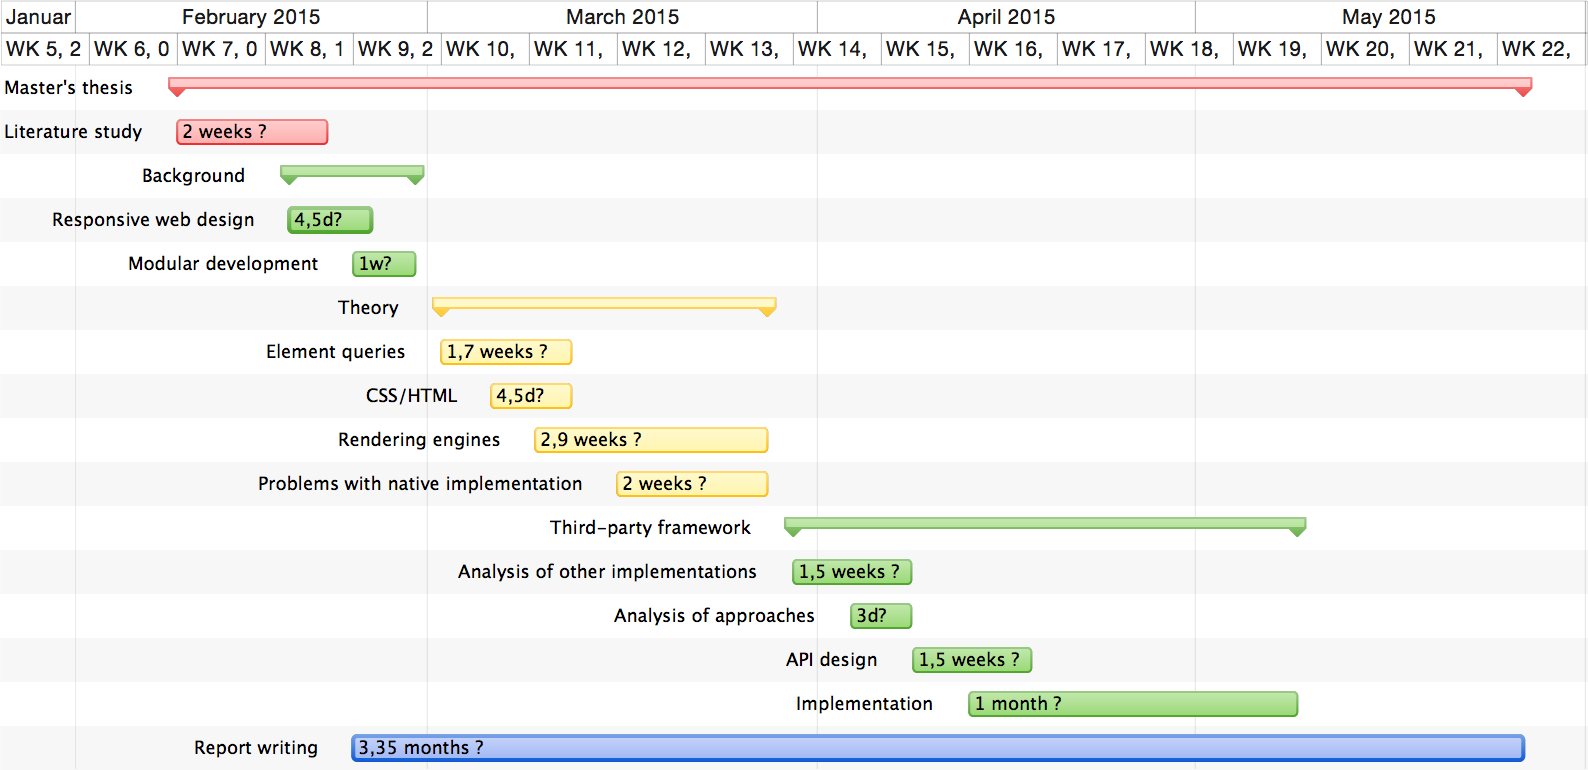
\includegraphics{timetable}
\caption{Box plot of number of positions sent per iteration using this scheme}
\label{fig:timetable}
\end{sidewaysfigure}
\restoregeometry

\end{document}
